
\section{Data}\label{Sec:Data}



%%%%%%%%%%%%%%%%%%%%%%%
%%%   Data source   %%%
%%%%%%%%%%%%%%%%%%%%%%%

\subsection{Source}\label{Sec:Data;Subsec:Source}

The data used for the present research was provided by Discovergy GmbH and can be downloaded from www.research.discovergy.com. Discovergy GmbH installs and maintains smart meters in German households for a one-time installation and monthly maintenance fee. Customers in return get various services centered around the analysis and visualization of their energy consumption and/or production. Discovergy describes itself as a full-range supplier of smart metering solutions offering transparent energy consumption and production data for private and commercial clients. All energy measurements of Discovergy smart meters are accessible through a web portal and mobile app. Additionally, various services are offered, such as, tips for energy savings potential, irregular consumption pattern warnings, personal energy reporting, and consumption analysis of individual appliances.

To be able to offer such data-driven services, Discovergy smart meters\footnote{Discovergy currently installs for private household clients the EasyMeter Q3D standard load profile meter which is connected to the Discovergy Meteorit TM smart meter gateway which records and transmits the recordings to Discovergy servers. The meter specifications can be found here: \texttt{https://discovergy.com/files/sources/product-information/SLP\_Zaehler.pdf} (in German).} record energy consumption and production near real-time -- i.e., 2-second intervals –- and send the readings to Discovergy's servers for storage and analysis. Therefore, Discovergy has extremely high resolution energy data of their customers at their disposal. This high resolution is in stark contrast to the half-hourly or even hourly recorded data used in previous studies (e.g., \cite{Arora:2016,Auder:2018,Shi:2017,Gerossier:2017}).

To the authors knowledge, there is no research using Discovergy smart meter data, apart from \cite{Teixeira:2017} who used the data as simulation input but not for analysis or prediction. As it was the first time that Discovergy provided data in this form for research purposes, there was no suitable process to retrieve data from their internal data storage solutions. For this reason, the author had to provide an API client for the Discovergy REST API to export data from pre-selected meters.


%%%%%%%%%%%%%%%%%%%%%%
%%%   Obtainment   %%%
%%%%%%%%%%%%%%%%%%%%%%

\subsection{Obtainment}\label{Sec:Data;Subsec:Obtainment}

As all Discovergy smart meters send their measurements in real-time to Discovergy\'s servers for storage, visualization and analysis, Discovergy clients can access their meters and measurements through a web application. Moreover, authorized users can interact with the stored meter measurements through predefined endpoints. These endpoints serve as an application programming interface (API) called Discovergy REST API. By providing the credentials for their Discovergy account\footnote{Sign up for a Discovergy account is open to everybody at https://my.discovergy.com/login. This provides access to the Discovergy API for developers, without the need of being a Discovergy client. However, only Discovergy clients will have access to smart meters in their account as their installed Discovergy meters are associated to their account.}, developers can send requests to a specified endpoint URL. The API returns to such a request a data object formatted in JavaScript Object Notation (JSON). For example, a user authenticates herself with her account credentials and requests the endpoint \texttt{GET /meters} at the base URL \texttt{https://api.discovergy.com/public/v1}. In response, the server returns a JSON object containing all meter IDs the user has access to.

To automate this process, the author of this study had to program an API client compliant with the constraints of a RESTful architecture.\footnote{REST refers to Representational State Transfer and describes an architetural style that ensures interoperability of systems through the web \citep[see][]{fielding:2000}.} This client  had to be able to authenticate the user with the provided account credentials, request the readings for one year in 3-minute intervals of all meters specified in a text file, and export them to a specified path. As the API had restrictions on the maximum time span of readings that could be returned depending on the measurement resolution (i.e., returns at most 10 days in 3-minute resolution), the client had to to make 37 request per meter to cover the whole year of 2017 in 10 day periods. As mentioned above, the measurement resolution of the Discovergy smart meters is with 2-second intervals much higher than the 3-minute intervals requested. However, the data management system employed by Discovergy already provides 3-minute aggregations of the original recordings which can be retrieved by specifying the according parameter in the API client.

The client was developed in Java based on the demo client provided in the Discovergy REST API documentation (https://api.discovergy.com/docs/). The client was then sent to an Discovergy employee who used an administrative account with access to a sufficiently large number of smart meters to retrieve the data sets used in this study. The code for the API client can be found in Appendix \ref{App:Code:C1API}.

%%%%%%%%%%%%%%%%%%%%%%%%%%%%
%%%   Data description   %%%
%%%%%%%%%%%%%%%%%%%%%%%%%%%%

\subsection{Description}\label{Sec:Data;Subsec:Description}

The data comes in 200 individual csv-files each containing the meter readings of a single smart meter. The readings are recorded in 3-minute intervals and range from 01.01.2017 00:00:00 to 01.01.2018 00:00:00. This translates into 175,201 observations per smart meter. Each smart meter measures energy consumption,  energy production (in the case of prosumers) and power over all phases installed in the meter and records them together with a timestamp in Unix milliseconds. For this research, only energy consumption and production are relevant. In summary, the data used here are 200 individual data sets each containing two time series (energy consumption and energy production) with 175,201 observations evenly spaced in 3-minute intervals.

Below, a preprocessed and correctly formatted sample of the data for consumer 56 and prosumer 89 containing 6 measurement points are shown.

\begin{table}[h]
    \csvreader[centered tabular=c|cc,
    table head=
    \hline\hline
    \textbf{time} & \textbf{energy} & \textbf{energyOut} \\
    \hline
    \ldots & \ldots & \ldots \\,
    head to column names,
    separator=comma,
    respect all,
    late after line=\\,
    table foot=
    \ldots & \ldots & \ldots \\\hline\hline]
    {tables/consumer-00000056_glimpse.csv}{}%
    {\csvcolii & \csvcoliii & \csvcoliv}%
    \caption[Data excerpt consumer 056]{Data excerpt consumer 056. \quantnet}
\end{table}

\begin{table}[h]
    \csvreader[centered tabular=c|cc,
    table head=
    \hline\hline
    \textbf{time} & \textbf{energy} & \textbf{energyOut} \\
    \hline
    \ldots & \ldots & \ldots \\,
    head to column names,
    separator=comma,
    respect all,
    late after line=\\,
    table foot=
    \ldots & \ldots & \ldots \\\hline\hline]
    {tables/producer-00000089_glimpse.csv}{}%
    {\csvcolii & \csvcoliii & \csvcoliv}%
    \caption[Data excerpt of prosumer 089]{Data excerpt consumer 089. \quantnet}
\end{table}

The energy and energy out measurements are recorded in the unit $10^{-10}$ kWh. As consumer 056 is not a prosumer and has no energy production capacity installed, all energy out measurements must be zero. Note however, that although the data excerpt of prosumer 089 shown here has positive energy out values, there may be prosumers with all zero energy out recordings if their production capacity never exceeds their own consumption. In this case the prosumer never actually feeds energy into the grid and the meter records a energy out reading of zero at all measurement points.



%%%%%%%%%%%
\subsubsection{Consumer data sets}


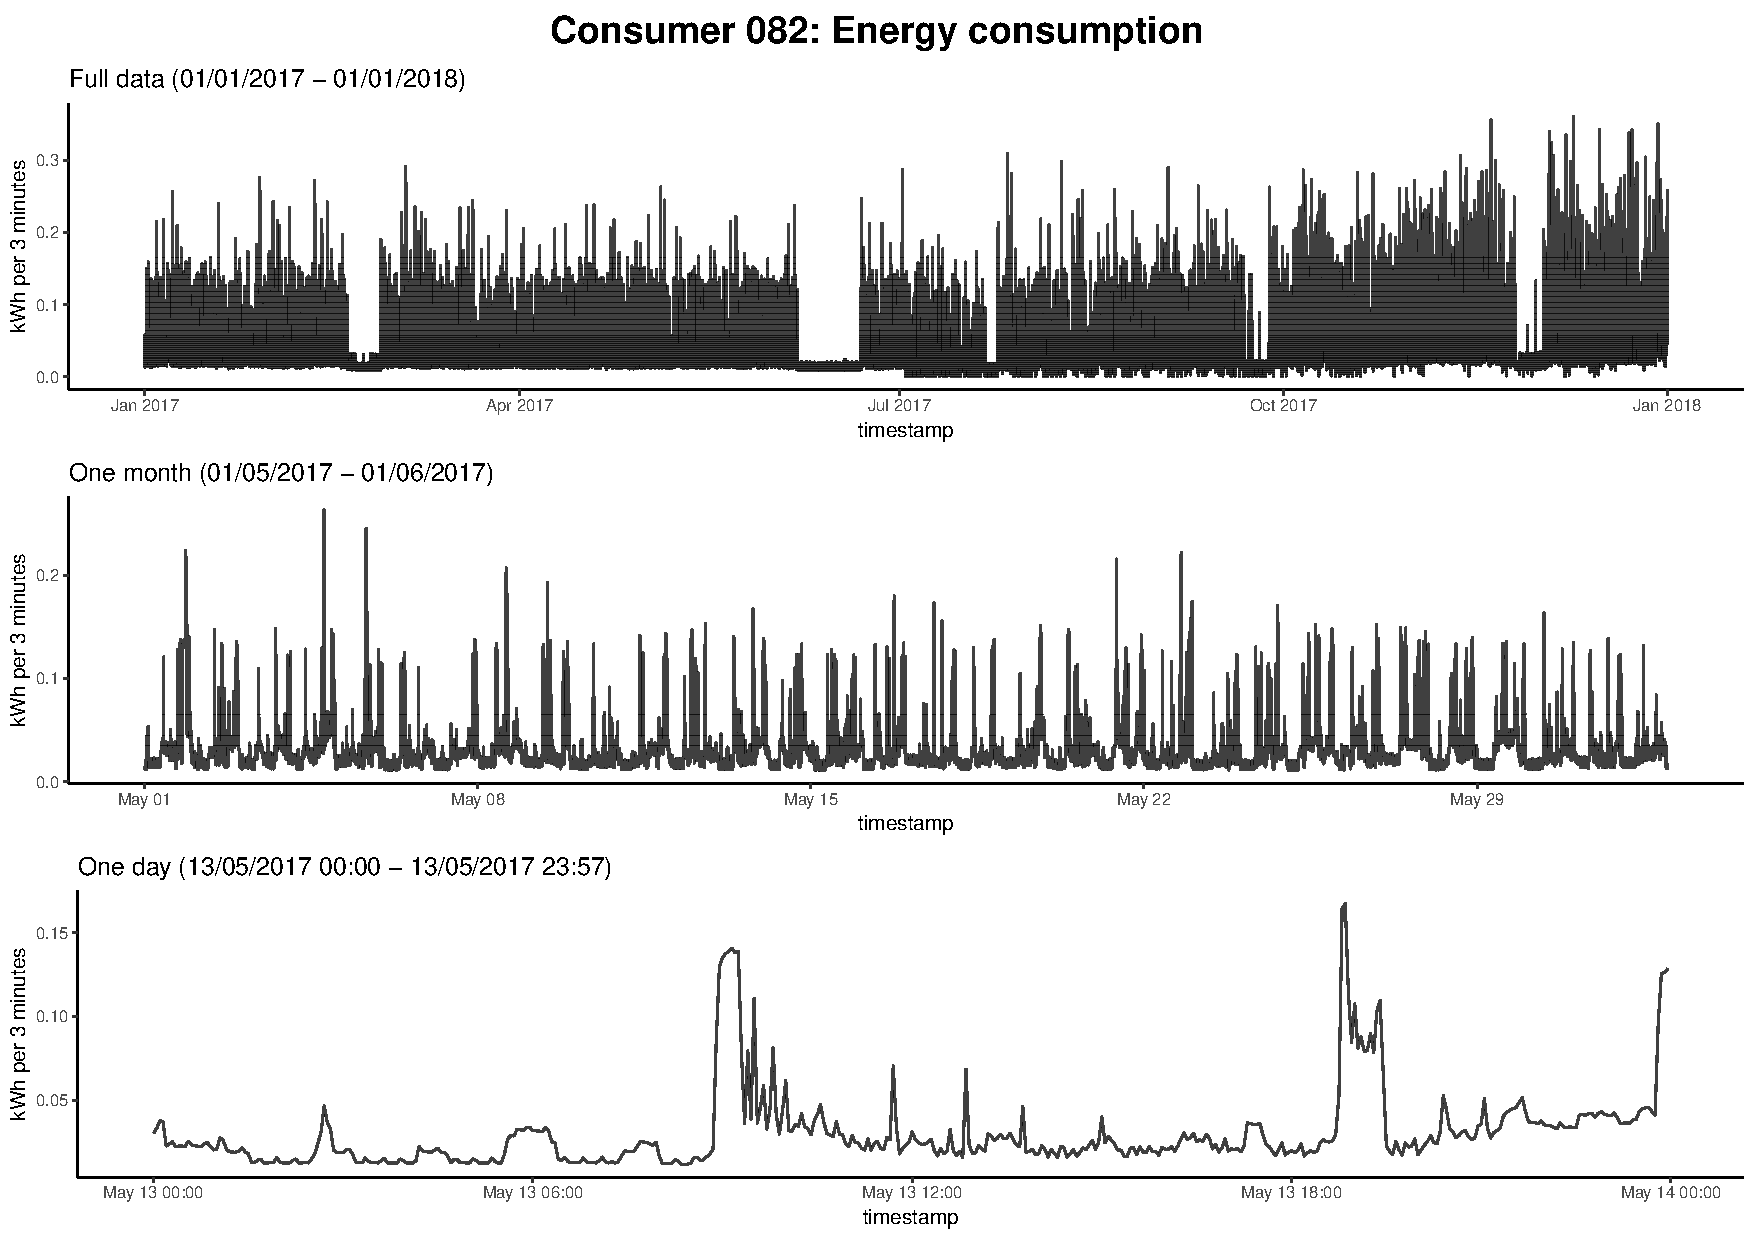
\includegraphics[width=\textwidth]{thesis/graphs/timeseries/c082_cons.pdf}\caption[]{Time series of energy consumption for consumer 082}



%%%%%%%%%%%
\subsubsection{Prosumer data sets}
%%%%%%%%%%%%%%%%%%%%%%%%%%%%%%%%%%%%%%%%%%%%%%%%%%%%%%%%%%%%%%%%%

\begin{itemize}

    \item Describe the data and its quality.
    \item How was the data sample selected?
    \item Provide descriptive statistics such as:
        \begin{itemize}
            \item time period,
            \item number of observations, data frequency,
            \item mean, median,
            \item min, max, standard deviation,
            \item skewness, kurtosis, Jarque--Bera statistic,
            \item time series plots, histogram.
        \end{itemize}
    \item For example:
        \begin{table}[ht]

        \begin{center}
            {\footnotesize
            \begin{tabular}{l|cccccccccc}
                \hline \hline
                           & 3m    & 6m    & 1yr   & 2yr   & 3yr   & 5yr   & 7yr   & 10yr  & 12yr  & 15yr   \\
                \hline
                    Mean   & 3.138 & 3.191 & 3.307 & 3.544 & 3.756 & 4.093 & 4.354 & 4.621 & 4.741 & 4.878  \\
                    StD    & 0.915 & 0.919 & 0.935 & 0.910 & 0.876 & 0.825 & 0.803 & 0.776 & 0.768 & 0.762  \\
                \hline \hline
            \end{tabular}}
        \end{center}
        \caption{Some descriptive statistics of location and dispersion for
        2100 observed swap rates for the period from February 15, 1999
        to March 2, 2007. Swap rates measured as 3.12 (instead of 0.0312). See Table
        \ref{Tab:DescripStatsRawDataDetail} in the appendix for
        more details.}
        \label{Tab:DescripStatsRawData}
        \end{table}

    \item Allows the reader to judge whether the sample is biased or to evaluate possible impacts of outliers, for
    example.

\end{itemize}
